\chapter{Acdt Framework}
\label{chap:Acdt_framework}

The section describes the implementation techniques employed for the parameters conversionand the fixing of t, c and both with not incremental or incremental calibration.

\section{Parameters conversion}

The following lines codify the conversion of the parameters:

\begin{lstlisting}
std::vector<Real> parameterConversion(std::vector<Real> coeff,std::vector<Real> guess, Real accuracy, Real min,Real max) const 
{
	Brent solver;
    //!The guess vector in this case is just a scalar "c"
	Real guess_ = guess[0];
	Real a = coeff[0], d = coeff[1], 
	sMax = coeff[2], tMax = coeff[3], c;
	//!Setup solver
	boost::function <Real(Rate)>error
	(boost::bind(&AbcdTenorBasis::parameterConversionError
	,this, _1, a, d, sMax, tMax));
	c = solver.solve(error, accuracy, guess_, min, max);
	//!return an acdt vector of coefficient
	return this->cadstToCoeff(c, coeff); 
}
\end{lstlisting} 

The function takes a guess of coefficients \{$a_{x}, d_{x}, s(t_{max}), t_{max}$\} and it outputs {$a_{x}, c_{x}, d_{x}, t_{max}$} or {$a_{x}, b_{x}, c_{x}, d_{x}$} according to the object, \textit{AcdtTenorBasis} or \textit{AbcdTenorBasis}, that invokes the function. 

Along with the coefficients it takes a guess vector. 
Despite the general interface in \textit{TenorBasis}:

\begin{lstlisting}
virtual std::vector<Real> parameterConversion(/*...*/)const = 0;
 \end{lstlisting}   
 
in case of abcd or acdt models it is simply a real scalar, because of b functional form, that implicitly fix b, only c is searched for.
In case of acdt it is only necessary to swap from $s(t_{max})$ to c, while in the abcd case, once obtained acdt, the vector needs to be converted through the functional form in abcd.

For achieving this result a solver is invoked and it is asked to zero the difference between the $s(t_{max})$ and it functional value.

Given \eqref{eqn:b_max} and \eqref{eq:s_x}, all the parameters of \textit{parameterConversionError} but c are fixed through \textit{boost::bind} and it is possible zeroing :

\begin{equation*}
s_{x}(t_{max})-\left(\frac{b_{x}}{c_{x}} e^{(\frac{a_{x}c_{x}}{b_{x}}-1)} +d_{x}\right)
\end{equation*}

changing and retrieving c.

\begin{lstlisting}
Real AbcdTenorBasis::parameterConversionError(const Real & c,const Real & a, const Real & d,const Real & sMax, const Real & tMax) const 
{
	Real b = (a*c) / (1 - tMax * c);
	//! s(t_max)- its functional form
	return sMax - ((b / c)*exp((a*c) / b - 1) + d);
}
\end{lstlisting} 

\section{Fixing of t, c and both with not incremental calibration}

In order to externally fix a parameter of a model is necessary an outer structure, such as the excel solver, which allows an inner calibration of the model while fixing its chosen parameters.

Transferring the \textit{TenorBasis} structure to this problem:

\begin{itemize}
    \item the external structure is created exploiting the QuantLib \textit{CalibratedModel} class, therefore \textit{TenorBasis} for the abcd / acdt framework and \textit{GlobalModel} here;
    
    \item the internal structure is created exploiting the QuantLib \textit{CalibrationHelperBase} class, therefore \textit{RateHelper} for the abcd / acdt framework and \textit{GlobalHelper} here.
\end{itemize}

Given that for using the \textit{GlobalModel} is necessary to build a \textit{GlobalHelper}, the latter is given the priority.

\subsection{Global Helper}

The \textit{GlobalHelper} class works as a wrap for the \textit{TenorBasis} model considerated. As explained in \eqref{chap:abcd_frame}, its function is required when the cost function in the minimize mechanism asks for the error.

\begin{lstlisting}

class GlobalHelper : public CalibrationHelperBase {
  public:
    GlobalHelper( const boost::shared_ptr<TenorBasis>& calibratedModel,
                  const std::vector<boost::shared_ptr<RateHelper>> & helpers,
                  boost::shared_ptr<OptimizationMethod> & method,
                  const EndCriteria  & endCriteria,
                  const std::vector<Real> & weights,
                  const std::vector<bool> & fixParameters);

    Real calibrationError()const;
    std::vector<boost::shared_ptr<RateHelper>>& getHelpers();
    boost::shared_ptr<OptimizationMethod>& getMethod();
    EndCriteria& getEndCriteria();
    std::vector<Real>& getWeights();
    std::vector<bool>& getFixParameters();
    boost::shared_ptr<TenorBasis> calibratedModel_;

  protected:
    std::vector<boost::shared_ptr<RateHelper>> helpers_;
    boost::shared_ptr<OptimizationMethod> method_;
    EndCriteria endCriteria_;
    std::vector<Real> weights_;
    std::vector<bool> fixParameters_;
}

\end{lstlisting}

The main method is \textit{calibrationError}. It is const because it is not modifying the \textit{GlobalHelper}, but just the \textit{TenorBasis} inside it as follows:

\begin{lstlisting}
Real GlobalHelper::calibrationError()const
{
   calibratedModel_->calibrate(helpers_, *method_, endCriteria_, weights_, fixParameters_);
   Array values = calibratedModel_->problemValues();
   Real value = 0;
   for (Size i = 0; i < values.size(); ++i) {
         value += values[i]* values[i];
   }
   return value;
}
\end{lstlisting}

Note that before retrieving the error the \textit{calibratedModel\_} is re-calibrated according to the new parameters generated in \textit{generateArguments}.

\subsection{Global Model}

As above explained, \textit{GlobalModel} is another implementation of \textit{CalibratedModel} with the peculiarity of using a \textit{GlobalHelper} as \textit{CalibrationHelperBase}:

\begin{lstlisting}
class GlobalModel : public CalibratedModel {
  public:
    GlobalModel(Size nArguments,
        const std::vector<Real>& coeff,
        const std::vector<boost::shared_ptr<GlobalHelper>> & helpers,
        const std::vector<Integer>& position);
    void generateArguments();
    virtual Constraint constraint() const;
    void calibrate(OptimizationMethod& method,
    
    const EndCriteria& endCriteria,
    const std::vector<Real>& weights,
    const std::vector<bool>& fixParameters);

  protected:
    std::vector<Integer> position_;
    std::vector<boost::shared_ptr<GlobalHelper>> helpers_;
}
 
\end{lstlisting}

The leading member functions are \textit{generateArguments} and \textit{calibrate}, but in order to make this object functional it is needed a trick. Considering that in the \textit{AcdtTenorBasis} and \textit{AbcdTenorBasis} classes it is possible to fix the parameter in order to make them simply scalar in the model, setting them as "TRUE" in \textit{GlobalHelper} and "FALSE" in \textit{GlobalModel} calibrate it allows to externally change the parameters while leaving internally the model to calibrate itself.

In the following \textit{generateArguments} is shown:

\begin{lstlisting}

void GlobalModel::generateArguments() 
{
    std::vector<Real> x(position_.size());
    for (Size i = 0; i < x.size(); ++i) {
        x[i] = arguments_[i](0.0);
    }
    
    for (Size j = 0; j < position_.size(); ++j) {
        for (Size i = 0; i < helpers_.size(); ++i) {
            //get parameters
            Array params = helpers_[i]->calibratedModel_->params(); 
            // set parameters of interest
            params[position_[j]] = x[j];
            // change model parameters
            helpers_[i]->calibratedModel_->setParams(params);
            }
         }
    }
}
    
\end{lstlisting}

The rationale is that given n parameters to be fixed there are n guesses that are copied from \textit{arguments\_} to x. Then, for each position in the vector \textit{position\_}, for each \textit{GlobalHelper} \textit{helpers\_} it asks the stored \textit{TenorBasis} its parameter, it changes the parameters in the j-th position with j-th \textit{x} vector entry and re-set  the \textit{TenorBasis} parameters with the new ones.

In the end the calibrate method:

\begin{lstlisting}
void GlobalModel::calibrate(OptimizationMethod& method,
                            const EndCriteria& endCriteria,
                            const std::vector<Real>& weights,
                            const std::vector<bool>& fixParameters)
{
    std::vector<boost::shared_ptr<CalibrationHelperBase>> 
    cHelpers(helpers_.size());
    for (Size i = 0; i < helpers_.size(); ++i){
        cHelpers[i] = helpers_[i];
        CalibratedModel::calibrate(cHelpers, method, endCriteria,
        this->constraint(), weights, fixParameters);
    }
}
       
\end{lstlisting}

mimics the calibrate \textit{TenorBasis::calibrate} method allowing the child class \textit{GlobalHelper} to be passed in place of the parent one \textit{CalibrationHelperBase}.

\subsubsection{Empirical test}
In order to test the goodness of the new methodology, given the same data sample, the acdt unconstrained calibration has been tested against abcd one:

\begin{figure}[H]
\centering
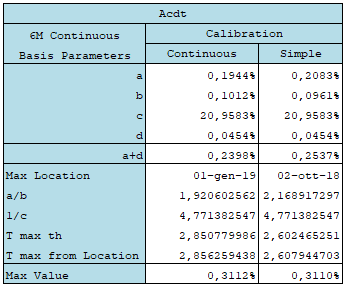
\includegraphics[scale=1]{acdt_vs_abcd_free_calib_acdt}
\caption{Acdt vs Abcd unconstrained calibration: Acdt (6M) }
\end{figure}

\begin{figure}[H]
\centering
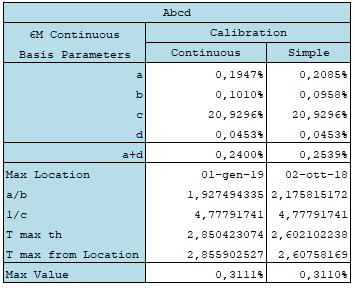
\includegraphics[scale=1]{acdt_vs_abcd_free_calib_abcd}
\caption{Acdt vs Abcd unconstrained calibration: Abcd (6M) }
\end{figure}

guaranteeing the exactness of the computational process.\footnote{The author guarantees for the exactness of each tenor based basis and invites the reader to look at the results available at his GitHub page: \url{https://github.com/GabrieleGiudic}}

